\documentclass[12pt, a4paper]{article}

\usepackage{fancyhdr, enumerate}
\usepackage{amssymb}
\usepackage{geometry, amsmath, amsfonts, float, graphicx}
\usepackage{gensymb}
\geometry{
	top=0.9in,           
	inner=0.6in,
	outer=0.6in,
	bottom=2in,
	tmargin= 10ex,       
	headsep=0.6cm,          
}
\pagestyle{fancy}

\fancyhead{}
\fancyfoot{}

\fancyhead[L]{Bioen 316 \\Homework 1: Part A\\ April 5, 2019}
\fancyhead[R]{Skyler Hallinan\\ hallisky@uw.edu \\ 1732227}


\begin{document}
\vspace*{-3mm}
\section*{Problem}
Given the given lead I and lead II voltages from Einthoven's Triangle (Figure 1), derive the formulas necessary to plot the heart’s electrical axis $V_H$ as a function of time. This heart electrical vector can be derived in cartesian or polar form..
\begin{figure}[h]
\caption{Einthoven's Triangle (from lecture)}
\centering
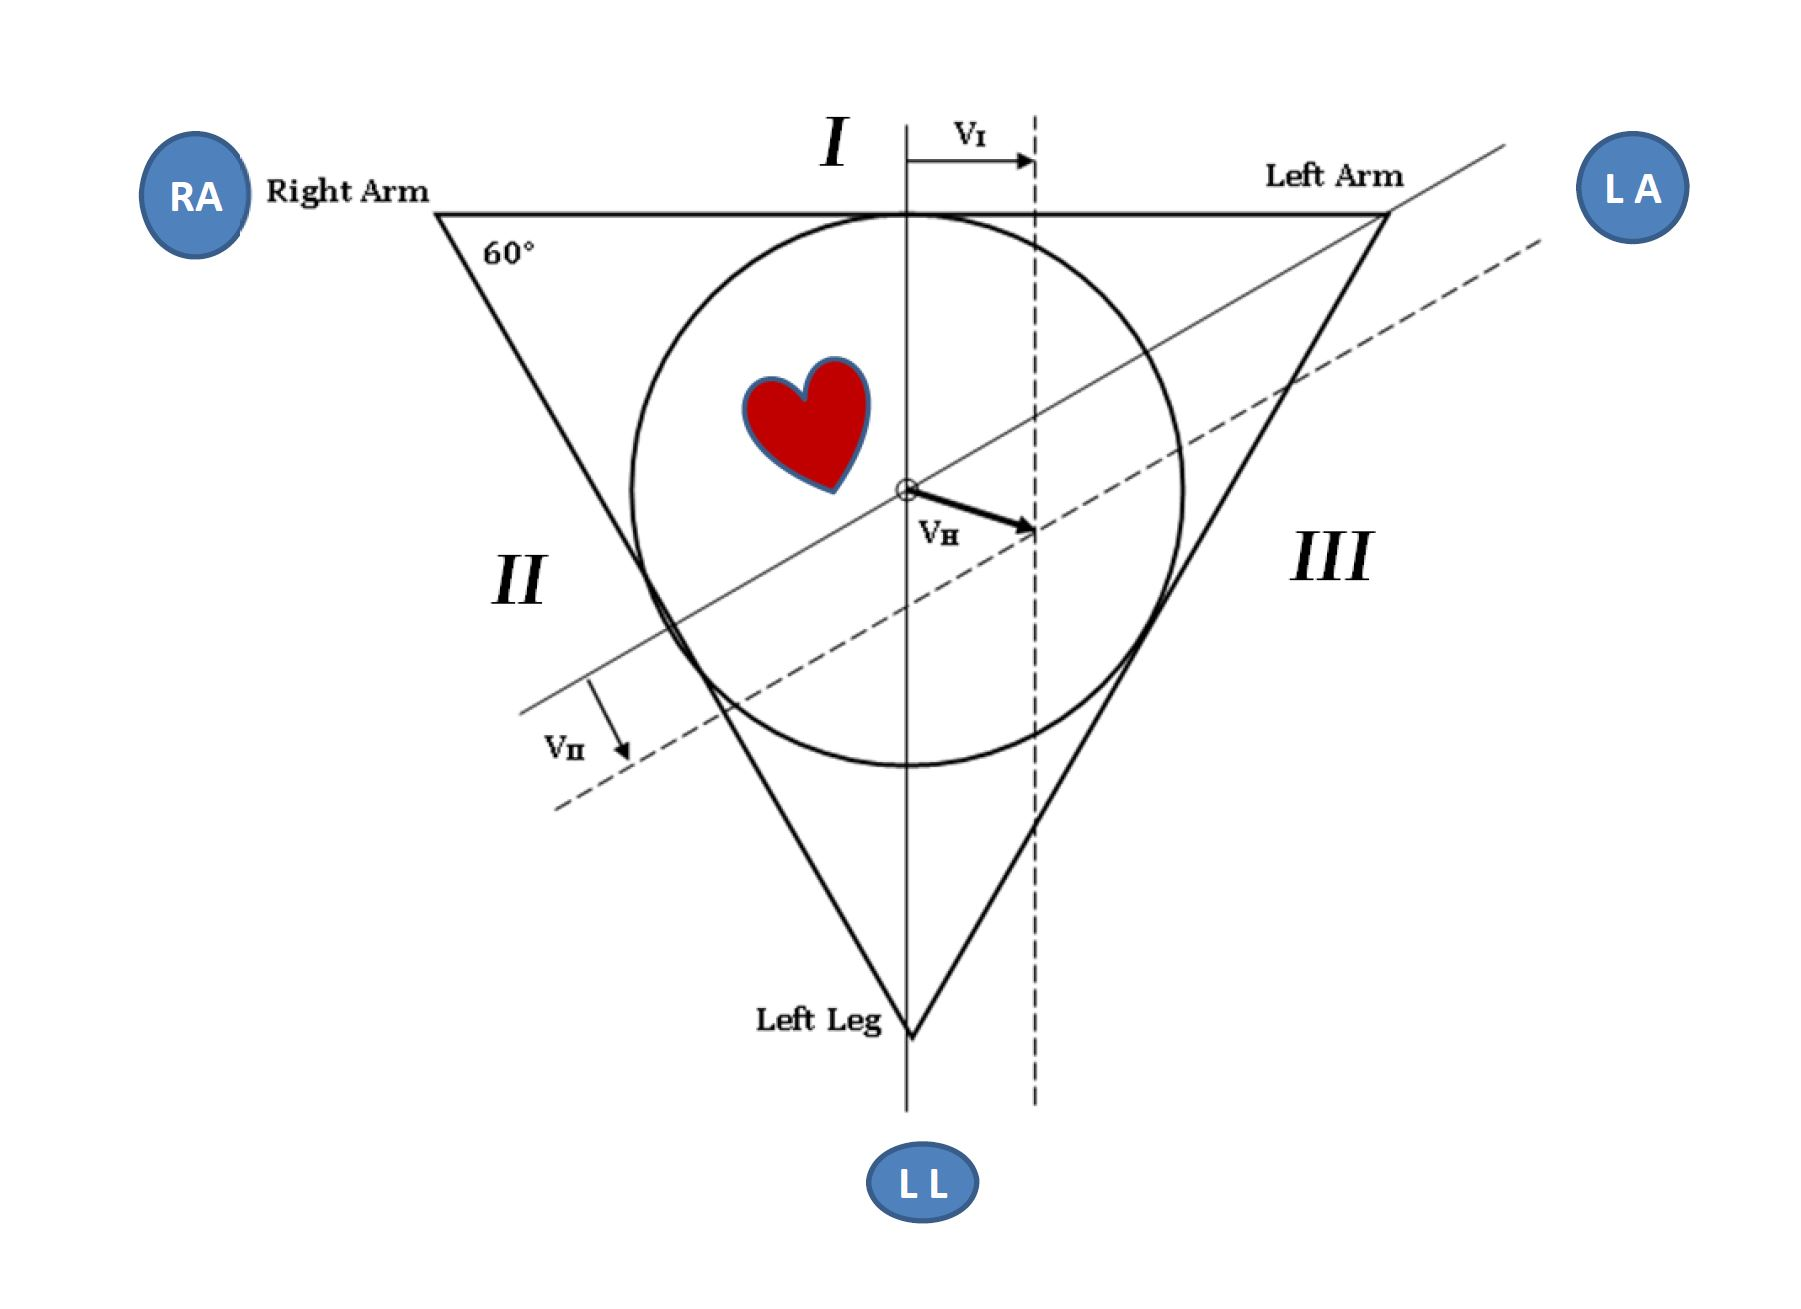
\includegraphics[width=0.9\textwidth]{heartdia}
\end{figure}
\pagebreak
\section*{Solution}
\begin{figure}[h]
\caption{Derivation of $V_H$ from Einthoven's Triangle}
\centering
\includegraphics[width=0.9\textwidth]{annotdiag.png}
\end{figure}
\noindent We are given the vectors $V_I$ and $V_{II}$ (as shown in both figures), and have to determine $V_H$ (also shown in the diagrams), for any magnitude conditions of $V_I$ and $V_{II}$. We first split our $V_H$ vector into its $x$ and $y$ components, $V_{Hx}$ and $V_{Hy}$. We will then determine these $x$ and $y$ components as shown in Figure 2. An important item to note is that although the magnitudes of $V_I$ and $V_{II}$ can potentially vary, the angles of these vectors are constant, since they are assumed to be set up in this Einthoven's Triangle configuration. Finally, when we refer to $V_I$ and $V_{II}$ in our following calculations, we will be refering to the \textbf{magnitude} of these vectors. These assumption is necessary for our following calculations. \\ \\
We first determine the value of $V_{Hx}$. We see from the figure that this value is equal to $V_I$; the $x$ component of this $V_H$ is completely independent of $V_{II}$, and instead depends entirely (and is equal to) $V_{I}$. Changing the magnitude of $V_{II}$ does not affect this $V_{Hx}$, while changing the magnitude of $V_I$ does. \\ \\
Calculations are a bit more complex to determine the $y$ component of the $V_H$ vector. The intersecting lines from the $V_I$ and $V_{II}$ vectors form a parallelogram inside Einthoven's Triangle. We will solve for the $y$ component of $V_H$ using the right side of this parallelogram. We first observe that Einthoven's Triangle is an equilateral triangle, so each angle in the triangle is 60\degree. We then note that the two lines extending perpendicularly from the endpoints of $V_{II}$ bisect the upper right vertex (the vector endpoint does in the figure), resulting in a 30\degree angle (from the perpendicular bisection), as labeled in Figure 2. We note that this 30\degree angle occurs even if this endpoint extends through the top edge of Einthoven's Triangle, not just when it goes straight through the upper right vertex. \\ \\
Then, using the vertical lines from $V_I$, we determine that in the small, upper right triangle made from the intersecting lines, we have a 30-60-90 \degree triangle; the vertical line from the 2nd endpoint of $V_1$ creates a 90\degree angle when it intersects the horizontal segment of the Einthoven's Triangle, so the final angle in the small triangle created by the intersections is 60\degree (angles sum to 180\degree). We then use vertical angles and parallel lines intersecting another line theorems to determine the angles in the rest of the figure. \\ \\
We see that the small triangle made in the left is another 30-60-90\degree triangle, with the 60\degree side length equaling $V_{II}$. Using the 1-$\sqrt{3}$-2 side lengths for this type of triangle, we determine that the side length of the 90\degree side is $\frac{2V_{II}}{\sqrt{3}}$. We see then that the side length of this parallelogram right side is equal to $\frac{2V_{II}}{\sqrt{3}}$, as it the same side length as the left side of the parallelogram, which we just computed. \\ \\
Finally, we solve for the right side of the small right triangle within the parallelogram. Through our theorems before (vertical angle and parallel lines intersecting another line), we have determined that this triangle is also a 30-60-90\degree triangle. We see that the bottom side, the 60\degree side, of this triangle equals $V_I$. Using the same logic as in the previous triangle, we determine the right side of this triangle to be $\frac{V_I}{\sqrt{3}}$. \\ \\ 
To obtain our final answers, we subtract this small side length from the total side length of the right side of the parallelogram to obtain the $y$ component of $V_H$. This gives us our $x$ and $y$ vector components of $V_H$. To convert to polar, we use the formulas $r = \sqrt{x^2 + y^2}$, $\theta = tan^{-1}(\frac{y}{x})$, where $r$ is the length of our  $V_H$ vector, and $\theta$ is the angle of it. We obtain the following answers:
\begin{align*}
\text{Cartesian: } V_{Hx} = V_I ,&\quad V_{Hy} =  \frac{2V_{II}}{\sqrt{3}} -\frac{V_I}{\sqrt{3}} \\
\text{Polar: } r = \sqrt{ V_I ^2 + (\frac{2V_{II}}{\sqrt{3}} -\frac{V_I}{\sqrt{3}})^2} ,&\quad \theta = tan^{-1}(\frac{\frac{2V_{II}}{\sqrt{3}} -\frac{V_I}{\sqrt{3}}}{V_I}) 
\end{align*}



\end{document}